% Survey - lista preliminar da literatura -> validação com usuários reais, agregando novos requisitos
% protocolo, questionário, requisitos propostos, resultados, análise

%=============================
\chapter{Survey}\label{survey}
%=============================

In this chapter, more detailed information is presented about the survey that was conducted. Similar to the previous chapter, which talks about the grey literature systematic review, the survey was also a joined effort work between two authors. The tasks on which each was responsible will be described later. \Cref{sec:survey-protocol}, presents details about the protocol created, author of reference and division of tasks among the researchers. Afterwards, in \Cref{sec:survey-validity}, threats to the validity of the study are reported. Finally, \Cref{sec:survey-results}, presents all results achieved during execution.

\section{Survey Protocol}\label{sec:survey-protocol}

According to \textcite{kasunic2005designing}, a survey is an approach to data collection and analysis in which participants answer questions or statements that were developed in advance. The protocol chosen for the elaboration of this study was also inspired by the guidelines proposed by the author and is illustrated in \Cref{fig:setepassos}.

\begin{figure}[!htb]
  \caption{Seven Steps of the Research Process}\label{fig:setepassos}
  \begin{center}
    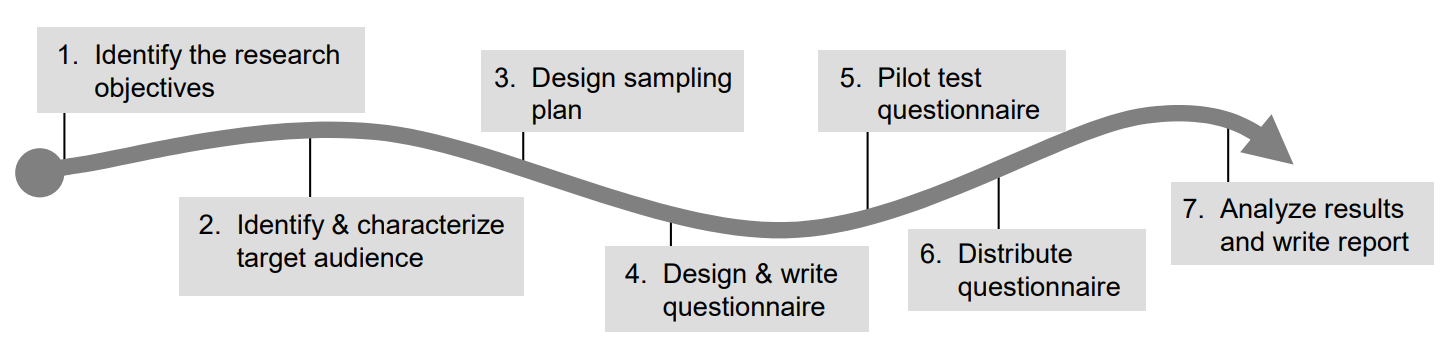
\includegraphics[width=16cm]{img/5-kasunic-process.png}
  \end{center}
  \fonte{\cite{kasunic2005designing}.}
\end{figure}

As will be described in more detail later, the objective is to understand the needs of students and teachers in relation to projects and outreach activities. The choice of a survey as a data collection approach is due to the fact that according to \textcite{kasunic2005designing}, the characteristics of such a research allows us to generalize about the beliefs and opinions of many people studying only a subset of them. Which is the perfect fit for this study.

Given that this research was performed by two students, the effort was divided equally, so that quality and performance were improved. \Cref{tbl:survey-tasks} describes the division of activities created by the authors and also already includes those defined by \textcite{kasunic2005designing}.

\begin{table}
  \centering
  \caption{Tasks Separation}
  \label{tbl:survey-tasks}
  \footnotesize
  \begin{tabular}{l|l}
    \bottomrule
    \rowcolor[rgb]{0.753,0.753,0.753} \multicolumn{1}{c|}{\textbf{Activity}}                             & \multicolumn{1}{c}{\textbf{Responsibility}} \\
    \hline
    \rowcolor[rgb]{0.898,0.898,0.898} Define and document research objectives                            & Lucas F.                                    \\
    Define and document research questions                                                               & Lucas F.                                    \\
    \rowcolor[rgb]{0.898,0.898,0.898} Define and document how research results will be used              & Lucas F.                                    \\
    Define the appropriate target audience for the research                                              & Igor C.                                     \\
    \rowcolor[rgb]{0.898,0.898,0.898} Determine the appropriate media to apply the research in           & Igor C.                                     \\
    Recruit members of the target audience to participate in pilot test                                  & Igor C.                                     \\
    \rowcolor[rgb]{0.898,0.898,0.898} Breakdown research questions into questionnaire topics             & Lucas F.                                    \\
    Organize and sequence questions                                                                      & Lucas F.                                    \\
    \rowcolor[rgb]{0.898,0.898,0.898} Review the questionnaire based on the pilot test                   & Igor C. and Lucas F.                        \\
    Perform the pilot test                                                                               & Igor C. and Lucas F.                        \\
    \rowcolor[rgb]{0.898,0.898,0.898} Evaluate comments                                                  & Igor C. and Lucas F.                        \\
    Perform final corrections before the distribution of the questionnaire                               & Lucas F.                                    \\
    \rowcolor[rgb]{0.753,0.753,0.753} \multicolumn{1}{c|}{\textbf{Questionnaire ready for distribution}} &                                             \\
    Distribute questionnaires                                                                            & Lucas F.                                    \\
    \rowcolor[rgb]{0.898,0.898,0.898} Monitor answers                                                    & Igor C. and Lucas F.                        \\
    Send reminders                                                                                       & Igor C.                                     \\
    \rowcolor[rgb]{0.753,0.753,0.753} \multicolumn{1}{c|}{\textbf{Questionnaire response deadline}}      &                                             \\
    Perform analysis                                                                                     & Igor C. and Lucas F.                        \\
    \rowcolor[rgb]{0.898,0.898,0.898} Write draft report                                                 & Igor C.                                     \\
    Revise draft                                                                                         & Igor C. and Lucas F.                        \\
    \rowcolor[rgb]{0.898,0.898,0.898} Perform the final corrections                                      & Igor C. and Lucas F.                        \\
    \toprule
  \end{tabular}
\end{table}

\subsection{Identify the Research Objectives}\label{sec:survey-objectives}

The point of having well defined research objectives, as \textcite{kasunic2005designing} presents, is to increase the odds of executing a successful questionnaire. Through the results generated by the grey literature systematic review, mentioned earlier in \Cref{greyliterature}, it was possible to elaborate questions so that the participant informs, in his view, the importance of a certain requirement. This survey aims to order by priority and refine the elicited requirements, using the individual opinion the target audience.

In addition to being asked the participants' opinion, they were also allowed to provide long written feedbacks and suggestions or improvements to each of the presented requirements. Since one of the objectives of the survey was to refine existing requirements, enabling the users to describe their thoughts in more detail allowed the authors to identify underlying issues that would otherwise go unnoticed.

\subsection{Identify and Characterize the Target Audience}\label{sec:survey-targets}

In this stage, an analysis is made to identify possible target groups and to properly select the one that best fits with the research. The population is also defined, and is composed by the academic community as a whole. To represent the population sample, the outreach program and project coordinators, teachers and students, with a preference for participants who have experience with outreach activities, were chosen.

\subsection{Design the Sampling Plan}\label{sec:survey-sampling}

According to \textcite{kasunic2005designing}, the purpose of this phase is to determine the following topics:
\begin{inparaenum}[(i)]
  \item How individuals will be selected to participate in the survey;
  \item The required size of the sample.
\end{inparaenum}

In order to select individuals to participate in the research, emails were sent to the Academic Secretariat of the \ac{UNIPAMPA} campuses, targeted to students and lists of outreach programs and projects coordinators. As expected, Uruguaiana and Bagé campuses, which executed the most outreach activities in 2021 \cite{relatorio-2021}, as seen in \Cref{fig:number-of-projects}, were the ones who provided the most respondents to the questionnaire.

\begin{figure}[!htb]
  \caption{Number of Projects Contemplated in the Internal Public Notices}\label{fig:number-of-projects}
  \begin{center}
    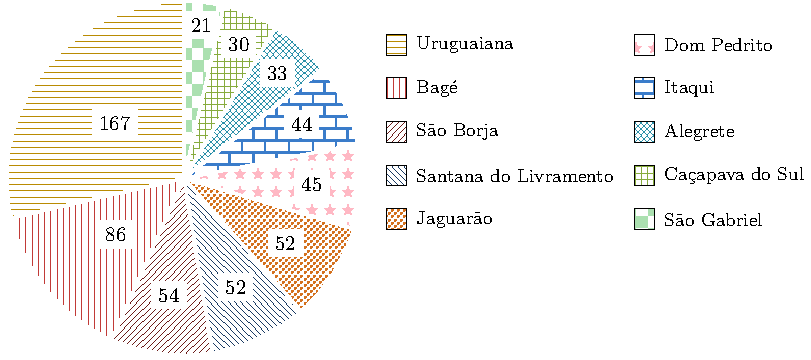
\includegraphics[width=16cm]{img/5-number-of-projects.pdf}
  \end{center}
  \fonte{Adapted from \textcite{relatorio-2021}}
\end{figure}

Besides all quantitative answers, each respondent had the opportunity to discuss in more depth about the presented questions, allowing for a qualitative feedback, which increased significantly the effort required to make the analysis. In total, the questionnaire had 123 responses.

Sample separation is an essential point for the best efficiency of the survey. The approach chosen was the number 22, defined by \textcite{Jefferson}, where the sample should be divided according to its characteristics and similarities. To implement it, the respondents of the questionnaire who declared themselves as \ac{ATE} or teachers were directed to one area of the questionnaire, and students to another, both areas with questions related to the responding profile.

\subsection{Design and Write the Questionnaire}\label{sec:survey-questionnaire}

According to \textcite[p. 34]{kasunic2005designing}, questions that do not have well defined goals are more likely to have questions that only consume time from the respondent, he emphasizes this with the following question: ``How can you reach insightful conclusions if you do not know what you were looking for or planning to observe?''

In this survey the goal is well defined, focused on prioritization of requirements and suggestions by possible end users as described in \Cref{sec:survey-objectives}. Similarly, the characteristics of the sample are important to write the questions in a way that everyone understands and not just the researchers. \textcite{surveyGuidelines} highlights that the results obtained with the survey are directly related to the quality of the questionnaire used.

For \textcite{surveyGuidelines} there are two types of questionnaires:
\begin{inparaenum}[(i)]
  \item self-administrated and
  \item interviewer-administrated questionnaires.
\end{inparaenum}
This one fits the first type, because it is a web-based questionnaire. The researches don't have to monitor the respondents. This model allows for more respondents, but on the other hand tends to have a higher dropout rate, emphasizing the importance of good structuring.

Google Forms was the chosen tool to create the questionnaire, since it contributes with a simple and uncluttered interface, while also being a part of the Google Suite service, which is adopted by \ac{UNIPAMPA} to support various processes, such as institutional emails, for example. It is also widely used, being familiar to much of the respondents. The form structure can be seen in \Cref{appendix:questionnaire}. The next sections will briefly describe each part of the questionnaire.

\subsubsection{The Welcome Section}\label{survey:welcome}

Following instructions from \textcite{kasunic2005designing}, the first page of the questionnaire contains important information for the participant, such as:

\begin{inparaenum}[(i)]
  \item Research objective;
  \item Estimated duration of the questionnaire;
  \item Researchers' contact email addresses;
  \item Researchers involved;
  \item Voluntary, anonymous and confidential character of the research;
  \item Institution and organization involved.
\end{inparaenum}

\subsubsection{Profile Questions}\label{survey:profile-questions}

The questions about the participant's personal information are important in the early stages of the questionnaire, as it motivates participants to continue answering the survey without asking complex questions early on \cite{LMRea}. In addition to a good classification of participants, it also allows the analysis of these to be done in a more controlled and organized way, as mentioned by \textcite{legramante}.

The profile questions asked are listed below:
\begin{inparaenum}[(1)]
  \item Is enrolled in \ac{UNIPAMPA};
  \item Gender;
  \item Age group;
  \item Academic education;
  \item Already participated in an \ac{OA};
  \item Which roles the participant had in the \ac{OA};
  \item His role in the academic community;
  \item His campus and city;
  \item The course the participant is taking.
\end{inparaenum}

\subsubsection{Requirements Prioritization Questions}

In questions related to the research objective, some directions described by \textcite{forza} were used, they are as follows:
\begin{inparaenum}[(1)]
  \item Define the way questions are asked to collect the information on a
  specific concept;\label{suggestion:1}
  \item For each question decide the scale on which the answers are placed;\label{suggestion:2}
  \item Identify the appropriate respondent(s) to each question;\label{suggestion:3}
  \item Put together the questions in questionnaires that facilitate and motivate the respondent(s) to respond.\label{suggestion:4}
\end{inparaenum}

\Cref{suggestion:1} suggests that the questions are written so that the entire responding sample can understand and formulate an answer. Since the questions of this questionnaire refer to software requirements, the user stories model has been used, which makes it very explicit who is the actor, what is desired with the requirement and the reason behind it. A user story can be defined as a casual, everyday summary of a software system's characteristics \cite{DIMITRIJEVIC2015352}. It was also determined that the questions would be classified as closed questions, where the possible answers are predetermined, as described by \textcite{forza}. However, at the end of each page, an open-ended question was also described, allowing the respondent to write freely whichever thoughts he had.

\Cref{suggestion:2} is about the scale used in the questions. At first the Likert scale \cite{joshi2015likert} would be used, but after better analysis, it was decided to use the an adapted \ac{MoSCoW} scale, which is widely used in requirements prioritization \cite{waters2009prioritization}.

Afterwards, \Cref{suggestion:3} says that the questionnaire should direct the participants to the questions they have more property to answer, bringing more constructive and relevant answers. This division was made using the profile questions commented in \Cref{survey:profile-questions}, where the participant is automatically directed to the section corresponding with his profile.

Finally, \Cref{suggestion:4} suggests that all questions that have a common subject should be organized near each other to facilitate cross checks between each other. To implement this, the requirements were grouped by the actors' roles, and they are:
\begin{inparaenum}[(1)]
  \item \ac{OA} proponent;
  \item \ac{OA} instructor;
  \item \ac{OA} participant;
  \item Outreach programs and projects coordinator.
\end{inparaenum}

The questions were also assigned \ac{ID} tags for each profile, in order to create better visualizations for the collected data later on. The logic behind the naming is simple. It starts with a letter which relates to the profile that that question is directed to, and a number, which is a simple count. They are as follows:
\begin{itemize}
  \item \textbf{A(1-14)}: ``A'' stands for ``Aluno'', the student or participant.
  \item \textbf{C(1-2)}: ``C'' stands for Coordinator.
  \item \textbf{I(1)}: ``I'' is for Instructor.
  \item \textbf{P(1-8)}: ``P'' stands for Proponent.
\end{itemize}
Students were directed to the A(1-14) questions, while professors and \acp{ATE} were directed to the remaining 3 categories, since they have a higher chance to perform any of these roles. The questions themselves will be described in more detail later on, in \Cref{ext:requirement-engineering}, when the system requirements are presented.

\subsubsection{Feature Suggestions}

For the last page of the questionnaire, a field was made available in which respondents may suggest to researchers any improvement, functionality, correction, anything they thought would be valuable for the goal product. With these answers it is possible to do a qualitative analysis and achieve new ideas for the development and completeness of the final tool.

\subsection{Pilot Questionnaire}\label{sec:survey-pilot}

As \textcite{kasunic2005designing} describes, a pilot test is a simulation of the real questionnaire carried out with a small number of members from the target audience. For this, the authors arbitrarily invited 7 (seven) people, out of which 4 (four) were students, 2 (two) were professors and 1 (one) was an \ac{ATE}. The reason behind choosing this specific number of respondents is due to the following:
\begin{inparaenum}[(i)]
  \item All defined profiles for the respondents were chosen and
  \item the ratio of 4/2/1 is aligned with the expected numbers of submitted questionnaires per profile.
\end{inparaenum}

Unfortunately, the person chosen for the third profile, \ac{ATE}, wasn't able to answer. However, even though there are 3 (three) profiles, the questionnaire itself only has 2 (two) tracks of questions, one for students and the other for professors/\acp{ATE}. Because of that, the consequences of this happening weren't too impactful.

As for the pilot results, a lot of great feedback was received, along with some compliments on the organization of the questionnaire. There were issues with the person identification section, where the age was changed from a number to a range of numbers, such as between 19-29 years old.

\subsection{Distribute the Questionnaire}\label{sec:survey-distribute}

The questionnaire was distributed to all people who make up the sample of this research. For this, first was collected all emails of coordinators with active outreach projects or programs, from several campuses of \ac{UNIPAMPA}. They were the first to respond the questionnaire.

After two (2) days, emails were sent to all campus academic secretariats, requesting that it be passed on to all the students from all courses. In total, the survey was open to answers for eighteen (18) days.

\subsection{Analyze the Results and Write a Report}\label{sec:survey-analyse}

The quantitative results related to the prioritization of requirements were collected and organized in graphs to better understand and visualize the data, while the qualitatives were subjectively analyzed and incorporated into the refined requirements list. Thus it will be possible to have an orderly list of requirements that were considered most important to end users, as well as well described user stories.

\section{Threats to Validity}\label{sec:survey-validity}

Validity is a critical variable in the success of a survey. Without the proper precautions, the whole study can fall apart if not carefully planned and executed. \textcite{kasunic2005designing} says that by following a well defined procedure and adapting it to fit the research subject, threats to the validity of the research can be avoided or minimized. The author cites two important types of validity in survey research:
\begin{inparaenum}[(1)]
  \item Construct validity and
  \item External validity.
\end{inparaenum}

The first item is about being certain of what is to be measured or collected. ``Are these questions providing enough information to answer my research objective?'' And the second validity is more about being able to generalize the obtained results to other people, places or times.

\subsection{Construct Validity}\label{sec:survey-construct-validity}

As soon as the first participants started submitting their responses, it was already possible to gather valuable information and insights from the results. That being said, the following items were identified as possible threats:
\begin{description}
  \item \textbf{1.} While the questions were simple and designed to be understood by everyone, the scale used, in the other hand, could be a cause of confusion by people who are not familiar with it. Even though the MoSCoW scale was adapted and translated to Portuguese, it could still be hard to answer for those who are not used to it.
  \item \textbf{2.} The questions were written in the form of user stories, making it easy for the participants to classify the relevance of the requirement. However, describing the questions this way could impose a threat in which the respondent might find difficult to suggest new functionalities, because the ``creative work'' was already done for them.
  \item \textbf{3.} The lack of clarity in definitions and amibiguity might also be considered threats. In some cases, the participant could not answer because he did not know what an \ac{OA} was.
\end{description}

\subsection{External Validity}\label{sec:survey-external-validity}

Regarding external validity, there are some inherent threats that come with how the scope of the study was defined. It is also impossible and unnecessary to completely neutralize this, as too much generalization would make the study less useful. Some of the threats were:
\begin{description}
  \item \textbf{1.} By the nature of the defined scope, the study is limited to participants which are familiar with the academic environment and preferably participated in an outreach activity in \ac{UNIPAMPA}.
  \item \textbf{2.} The scope could be expanded to other \ac{HEI} without adding much risks, but then the study would become less useful, since this term paper describes a goal product directed at \ac{UNIPAMPA}.
\end{description}

\section{Results}\label{sec:survey-results}

In the 18 days that the questionaire was available for responses, 123 responses from students, teachers, and \acp{ATE} were collected. As all of the quantitative questions had an obligatory nature, a response rate of 100\% was obtained for each respondent's profile. On the other hand, when all of the qualitative questions were answered, including those on the final page of the questionnaire and those asking for general suggestions for the tool, the percentage of responses from teachers and students was approximately 23\% and 12\%, respectively. This low value was one of the factors contributing to the validity threat mentioned in Item 3 of \Cref{sec:survey-construct-validity}.

The charts related to participant identification and their participation in outreach academic activities will be presented in the following section, \Cref{sec:survey-participant-id}. The results obtained in objective and quantitative questions where the \ac{MoSCoW} requirement prioritization technique was applied are described in \Cref{sec:survey-quant}. Last but not least, in \Cref{sec:survey-quali}, the final ranking of the requirements based on the respondents' written and qualitative feedback as well as their most pertinent suggestions will be presented.

% Charts source https://www.overleaf.com/read/fkzhpvsnsfhx

\subsection{Respondent Identification}\label{sec:survey-participant-id}

This section presents information pertaining to the respondent profile and the survey's demographic is depicted. \Cref{fig:sex-distribution} and \Cref{fig:age-distribution} show that most of the respondents identify as the female gender, while also being within the 19-39 age ranges. This information is relevant to understand the demographic, which is comprised mostly by college students, as can be seen in \Cref{fig:formation-distribution} and \Cref{fig:community-roles}.

Another important piece of information obtained through analyzing the identification results is the city and campuses most respondents come from. As it was shown earlier in \Cref{fig:number-of-projects}, more students from Uruguaiana - the campus which executed most \aclp{OA} in 2021 - were expected to respond, which was not the case, as can be seen in \Cref{fig:city-distribution}.

Lastly, it is presented the charts regarding the participation of respondents in \acp{OA}. \Cref{fig:outreach-participation} shows an interesting result. Over a quarter of respondents have never participated, not even as listeners, in an \ac{OA}. This posed a possible threat, described in items 2 and 3 of \Cref{sec:survey-construct-validity}. Finally, \Cref{fig:outreach-roles} aims to map the roles each respondent had when participating in \acp{OA}. Over half of them had participated as listeners.

\begin{figure}[!htb]
  \caption{Participants Gender Distribution}\label{fig:sex-distribution}
  \begin{center}
    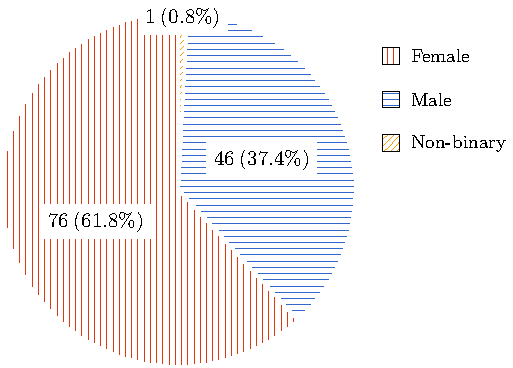
\includegraphics[width=9cm]{img/5-participants-sex.pdf}
  \end{center}
  \fonte{Author.}
\end{figure}

\begin{figure}[!htb]
  \caption{Participants Age Distribution}\label{fig:age-distribution}
  \begin{center}
    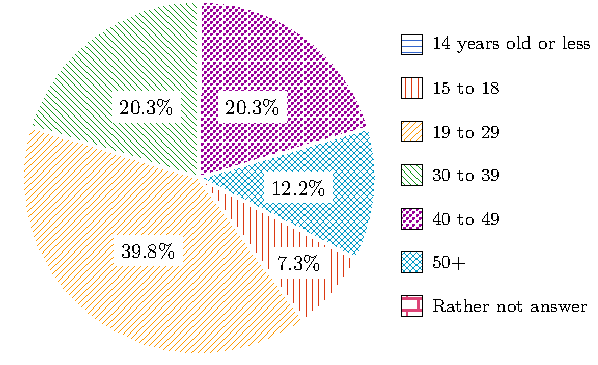
\includegraphics[width=9cm]{img/5-participants-age.pdf}
  \end{center}
  \fonte{Author.}
\end{figure}

\begin{figure}[!htb]
  \caption{Participants Formation Distribution}\label{fig:formation-distribution}
  \begin{center}
    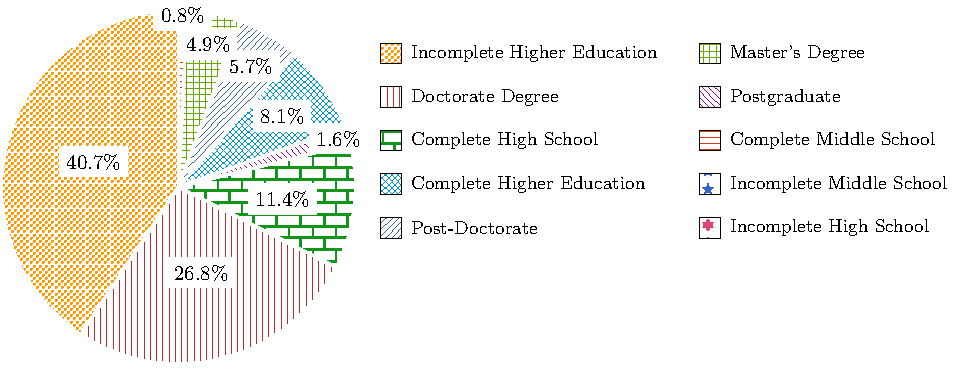
\includegraphics[width=14cm]{img/5-participants-formation.pdf}
  \end{center}
  \fonte{Author.}
\end{figure}

\begin{figure}[!htb]
  \caption{Community Roles Distribution}\label{fig:community-roles}
  \begin{center}
    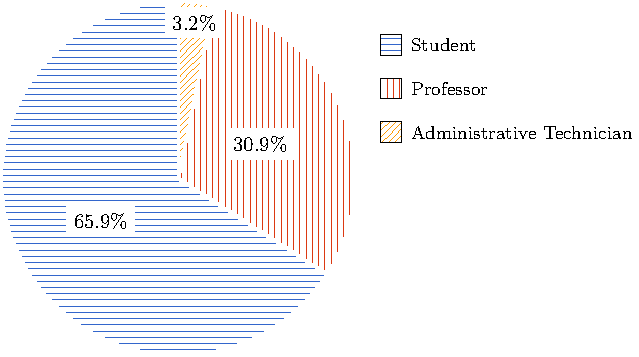
\includegraphics[width=9cm]{img/5-community-roles.pdf}
  \end{center}
  \fonte{Author.}
\end{figure}

\begin{figure}[!htb]
  \caption{Participants City Distribution}\label{fig:city-distribution}
  \begin{center}
    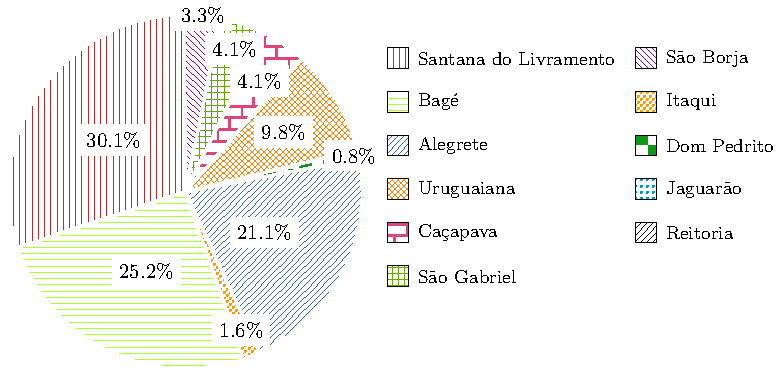
\includegraphics[width=12cm]{img/5-participants-city.pdf}
  \end{center}
  \fonte{Author.}
\end{figure}

\begin{figure}[!htb]
  \caption{Outreach Participation Distribution}\label{fig:outreach-participation}
  \begin{center}
    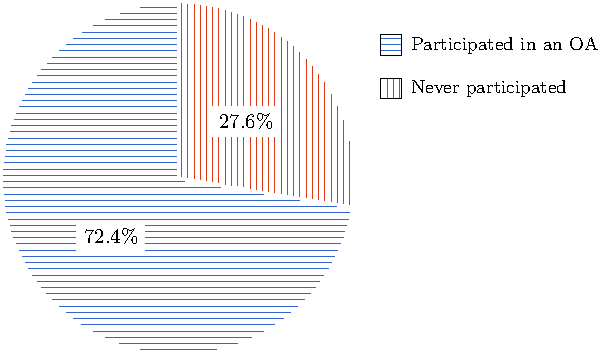
\includegraphics[width=9cm]{img/5-outreach-participation.pdf}
  \end{center}
  \fonte{Author.}
\end{figure}

\begin{figure}[!htb]
  \caption{Outreach Roles Distribution}\label{fig:outreach-roles}
  \begin{center}
    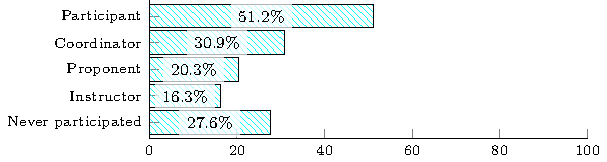
\includegraphics[width=13cm]{img/5-outreach-roles.pdf}
  \end{center}
  \fonte{Author.}
\end{figure}

\subsection{Quantitative Results}\label{sec:survey-quant}

The quantitative results were gathered by asking objective questions in which the respondant had to prioritize the user story in the question using the MoSCoW scale, described earlier.

By analyzing the results obtained in each of the questions asked in the questionnaire, which is available at \Cref{appendix:questionnaire}\footnote{As a note, to better navigate from the charts to the questions themselves, which are all the way down in the appendix, open the PDF in the browser and hit ``CTRL + F'', searching for the question \ac{ID} and using the arrows to navigate between occurrences.}, some interesting results were found regarding each user role defined for the \ac{MVP}, which are going to be discussed later in more detail in \Cref{ext:initial-considerations}. The following sections describe the results obtained on each of their quantitative questions. The roles are as follows:
\begin{inparaenum}[(a)]
  \item Proponent,
  \item Coordinator,
  \item Instructor and
  \item Participant.
\end{inparaenum}

\subsubsection{Proponent}\label{sec:survey-quant-proponent}

Regarding the proponent role, the results collected were a success. The presented written survey questions identified by P(1-8) were on point, with most of them scoring Musts and Should haves as it can be seen in \Cref{fig:proponent-questions}, meaning they are great features which the future target users would like to see in the system. The only exceptions were P2 and P5, scoring the most of Could and Will not haves out of all of the questions.

A sub question of the user story described by P7 can be seen in \Cref{fig:p7-question}. The respondents could check both alternatives for communicating with the future \ac{OA} participants, and it was unexpected that \textit{WhatsApp} got over half of votes, considering the history of using emails most of the time for communication in the university.

\begin{figure}[!htb]
  \caption{Questions Regarding Proponent Role}\label{fig:proponent-questions}
  \begin{center}
    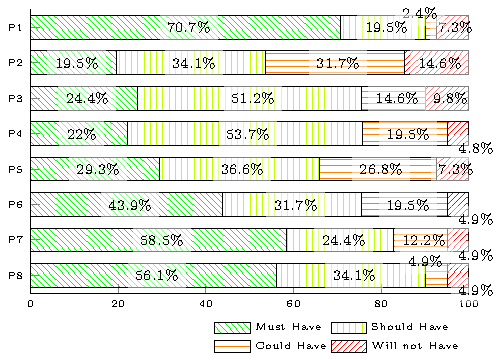
\includegraphics[width=13cm]{img/5-questions-proponent.pdf}
  \end{center}
  \fonte{Author.}
\end{figure}

\begin{figure}[!htb]
  \caption{Which communication channel the proponent prefers}\label{fig:p7-question}
  \begin{center}
    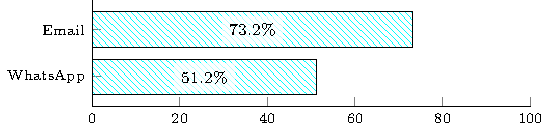
\includegraphics[width=13cm]{img/5-questions-proponent-P7-1.pdf}
  \end{center}
  \fonte{Author.}
\end{figure}

\subsubsection{Coordinator}\label{sec:survey-quant-coordinator}

Not many questions were asked about this user role. It was interesting to see the first question, C1, not receiving as much Must haves as C2, since it was assumed that the review and approval process of \acp{OA} was as much if not more important than issuing participation certificates. The results can be seen in \Cref{fig:coordinator-questions}.

\begin{figure}[!htb]
  \caption{Questions Regarding Coordinator Role}\label{fig:coordinator-questions}
  \begin{center}
    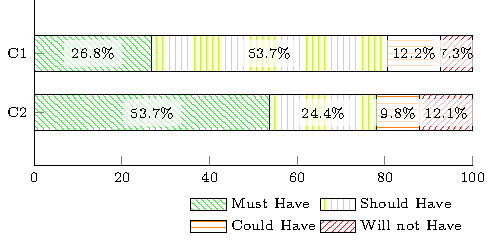
\includegraphics[width=13cm]{img/5-questions-coordinator.pdf}
  \end{center}
  \fonte{Author.}
\end{figure}

\subsubsection{Instructor}\label{sec:survey-quant-instructor}

As it was realized before, the survey respondents value greatly the issuance of participation certificates. The same can be said for the only question regarding the Instructor role, which can be seen in \Cref{fig:instructor-questions}. Having over 60\% Must haves, it's one of the user stories with highest priority in the study.

\begin{figure}[!htb]
  \caption{Questions Regarding Instructor Role}\label{fig:instructor-questions}
  \begin{center}
    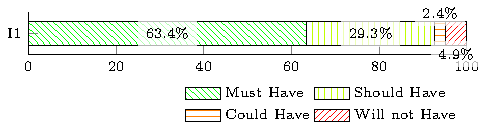
\includegraphics[width=13cm]{img/5-questions-instructor.pdf}
  \end{center}
  \fonte{Author.}
\end{figure}

\subsubsection{Participant}\label{sec:survey-quant-participant}

This is where most of the survey demographics was directed to. Since all of the students were chosen to respond only to the participant system user role, while the professors and \acp{ATE} answered for three different profiles, a balanced number of questions was aimed for. In total, students had 14 questions, while teachers and \acp{ATE} had 11.

The results are divided in two charts, the first can be seen in \Cref{fig:participant-1} and presents the first 1-7 questions, while the second, shown in \Cref{fig:participant-2} displays the last 8-14 questions. It was great to see the respondents prioritizing most of the user stories as Must haves, especially the first seven (7), meaning the requirements were once again well described and important for the system. However, not all of them were ranked highly, such as A11 and A13, which showed an above average number for Could and Will not haves.

A11 makes sense, since it could be hard to think as someone who is not enrolled in the university. This user story is also a little bit of out scope for an \ac{MVP}, so the feedback was important to rank it lower in the requirements. A13 was a bold feature, which came up during a brainstorm with the supervisor. It's interesting to see it wasn't as exciting for the respondents as it was when the idea of assigning grades to \acp{OA} was conceived.

Lastly, A14 had a sub question, similar to P7, in which respondents should choose where they would rather see the upcoming \acp{OA} they were enrolled in. Implementing a calendar view in the website itself could be very time consuming, so it was great to know beforehand that the majority of users would rather export the \ac{OA} to their own calendar apps.

\begin{figure}[!htb]
  \caption{Questions Regarding Participant Pt.1}\label{fig:participant-1}
  \begin{center}
    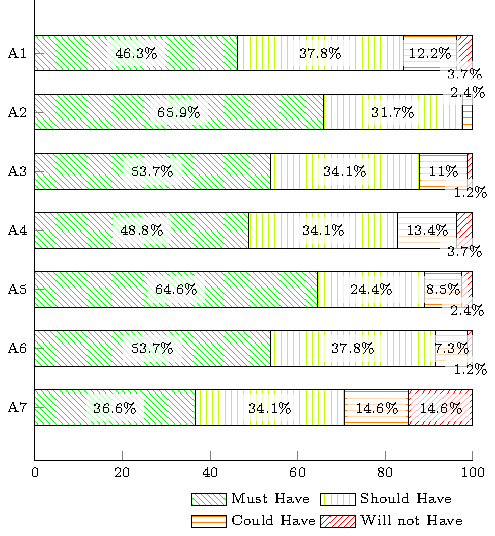
\includegraphics[width=13cm]{img/5-questions-participant-1.pdf}
  \end{center}
  \fonte{Author.}
\end{figure}

\begin{figure}[!htb]
  \caption{Questions Regarding Participant Pt.2}\label{fig:participant-2}
  \begin{center}
    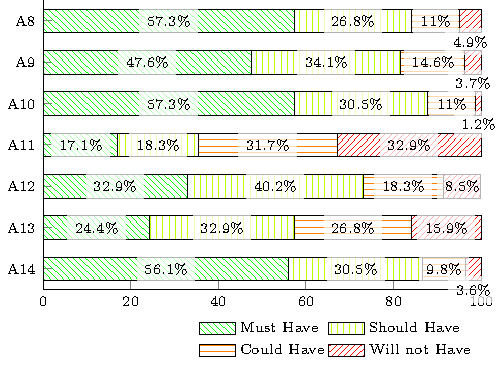
\includegraphics[width=13cm]{img/5-questions-participant-2.pdf}
  \end{center}
  \fonte{Author.}
\end{figure}

\begin{figure}[!htb]
  \caption{Where the user would rather see their upcoming \ac{OA}}\label{fig:participant-a14}
  \begin{center}
    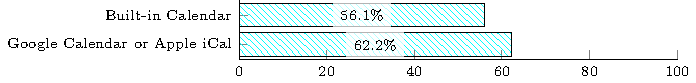
\includegraphics[width=13cm]{img/5-questions-participant-A14-1.pdf}
  \end{center}
  \fonte{Author.}
\end{figure}

\subsection{Qualitative Results}\label{sec:survey-quali}

Regarding the written feedback respondents were free to write in each page, most of them were short and somewhat out of scope, saying things that were already said in the questions and compliments about the iniciative of doing this study. However, a few of them were very useful feedback, presenting critics of the present way of doing things and expanding the knowledge of the authors by explaining more about the respondent's individual experiences.

The responses will be translated freely from their original language, Portuguese, and described below.

As expected, there was a lot of differences between students' feedbacks and professors/\acp{ATE} feedbacks. Most relevant ones were written by teachers and \acs{ATE}, which will be discussed in more detail briefly. The following, however, are judged to be noteworthy feedbacks by students:
\begin{itemize}
  \item  ``\textit{Regarding A9, it would be cool to send out notifications, for instance, when an \ac{OA}'s registration deadline is approaching}''. This was a very interesting and valid suggestion, which, besides the notifications part, opens doors to features such as having an \ac{OA} watchlist and saving favorites.
  \item ``\textit{The questions are repetitive, leading the individual to declare them irrelevant}''. This was unexpected input on the survey's questions because it wasn't raised at any point during the survey's development. Nevertheless, it was excellent feedback.
  \item ``\textit{Change the order of importance and the highest level of satisfaction since the order of presentation of the points was incorrect at the beginning of the question because it starts with number 4}''. Maybe setting the MoSCoW scale in reverse, starting with Must Have as a 1, instead of a 4, would add more value. However, this was the only criticism written on this topic.
\end{itemize}

Next are the noteworthy feedbacks received by professors and \acp{ATE}:
\begin{itemize}
  \item Two respondents raised the topic of work and the volume of information to be provided as one of their points. They emphasize that because outreach activities must currently be recorded in the \ac{SAP} project, it is crucial that the final tool be able to provide a report in the format accepted by this tool; otherwise, teachers would have to complete more work in both tools. One of them also points out that it would be much more interesting the forms in the tool were as succint as possible, as this would make preenchiment easier and add less burocratic burden.
  \item Another important point to keep in mind is that participants who have a history of absenteeism or low participation in the activities in which they are registered are abusing their slots. It was suggested as a solution to this that the system be aware of these people and give them less priority than someone who is on time for their commitments when they are placed in a line for registration for an \ac{OA}.
  \item A concern raised by a coordinator of outreach activities is the generation of \ac{PROEXT} certificates that frequently do not provide the estimated time of return to the coordinator. For this reason, participants who are unsure of how this procedure works end up asking the coordinator instead of the actual \ac{PROEXT}, which is inconvenient. He suggests sending notifications or perhaps a visualization tool that provides information on the expected date for certificate generation.
  \item According to a professor, the generation of presence certificates is currently done one by one on the \ac{SEI}, and this process is very slow. He suggests speeding up the procedure so that all of the certificates can be generated at once. Another respondent claims that the possibility of generating presence certificates without having to wait for the \ac{OA} completion date would be interesting, particularly for the external public.
\end{itemize}

\section{Chapter Summary}\label{survey:chapter-summary}

In this chapter, the survey as a whole was discussed, describing points such as details about the followed protocol, strategies used in developing the questions, threats to validity and both quantitative and qualitative analysis of the results obtained. \Cref{extensionly} will discuss more about the specifics of the Front-end \ac{MVP} developed, presenting about pertinent design decisions.